% IF YOU CAN SEE THIS GO CONTRIBUTE >:(

\documentclass[letterpaper, 8pt]{extarticle}
\usepackage{amssymb,amsmath,amsthm,amsfonts}
\usepackage{multicol,multirow}
\usepackage{calc}
\usepackage{ifthen}
\usepackage[landscape]{geometry}
\usepackage[colorlinks=true,citecolor=blue,linkcolor=blue]{hyperref}

\usepackage{booktabs}
\usepackage{ulem}
\usepackage{enumitem}
\usepackage{tabulary}
\usepackage{graphicx}
\usepackage{siunitx}
\usepackage{tikz}
\usepackage{derivative}
\usepackage{svg}
\usepackage{listings}
\usepackage{setspace}
\usepackage{listings}
\usepackage{xcolor}
\usepackage{courier}

% minimal line spacing
\setstretch{0.1}

% set borders (experimentally determined to minimize cutoff and maximize space on school printers)
\geometry{top=.25in,left=.25in,right=.25in,bottom=.35in}

% make figures work better in multicol
\newenvironment{Figure}
{\par\medskip\noindent\minipage}
{\endminipage\par\medskip}

\pagestyle{empty} % clear page

% rewrite section commands to be smaller
\makeatletter
\renewcommand{\section}{\@startsection{section}{1}{0mm}%
                                {-1explus -.5ex minus -.2ex}%
                                {0.5ex plus .2ex}%x
                                {\normalfont\normalsize\bfseries}}
\renewcommand{\subsection}{\@startsection{subsection}{2}{0mm}%
                                {-1explus -.5ex minus -.2ex}%
                                {0.5ex plus .2ex}%
                                {\normalfont\small\bfseries}}
\renewcommand{\subsubsection}{\@startsection{subsubsection}{3}{0mm}%
                                {-1ex plus -.5ex minus -.2ex}%
                                {1ex plus .2ex}%
                                {\normalfont\tiny\bfseries}}
\makeatother
\setcounter{secnumdepth}{0} % disable section numbering

% disable indenting
\setlength{\parindent}{0pt}
\setlength{\parskip}{0pt plus 0.5ex}

% Custom siunitx defs
\DeclareSIUnit\noop{\relax}
\NewDocumentCommand\prefixvalue{m}{%
\qty[prefix-mode=extract-exponent,print-unity-mantissa=false]{1}{#1\noop}
}

% Shorthand definitions
\newcommand{\To}{\Rightarrow}
% holy fck thanks for this
\newcommand{\ttt}{\texttt}

% condense itemize & enumerate
\let\olditemize=\itemize \let\endolditemize=\enditemize \renewenvironment{itemize}{\olditemize \itemsep0em}{\endolditemize}
\let\oldenumerate=\enumerate \let\endoldenumerate=\endenumerate \renewenvironment{enumerate}{\oldenumerate \itemsep0em}{\endoldenumerate}
\setlist[itemize]{noitemsep, topsep=0pt, leftmargin=*}
\setlist[enumerate]{noitemsep, topsep=0pt, leftmargin=*}

\title{3SH3}

\begin{document}
% \raggedright
\tiny

% make listings look nicer
\lstset{
    tabsize = 2, %% set tab space width
    showstringspaces = false, %% prevent space marking in strings, string is defined as the text that is generally printed directly to the console
    basicstyle = \tiny\ttfamily, %% set listing font and size
    breaklines = true, %% enable line breaking
    numberstyle = \tiny,
    postbreak = \mbox{\textcolor{red}{\(\hookrightarrow\)}\space}
}

\begin{center}
    {\textbf{3SH3 Final -- Linus Torvalds Edition}} \\
\end{center}
% set column spacing rules
\setlength{\premulticols}{1pt}
\setlength{\postmulticols}{1pt}
\setlength{\multicolsep}{1pt}
\setlength{\columnsep}{2pt}
\begin{multicols*}{6}
    % sections based on slide titles
    \section{Overview}
    \textbf{System Programs:} associated with the operating system but are not
    necessarily part of the kernel.\\
    \textbf{Middleware:} software frameworks that provide additional services to
    application developers.
    \section{Processes}
    \textbf{Possible states of a process}: new, running, waiting, ready,
    terminated.
    \subsection{Process Creation Code}
    \begin{lstlisting}[language=C]
int main()
{
    pid t pid;
    /* fork a child process */
    pid = fork();
    if (pid < 0) { /* error occurred */
        fprintf(stderr, "Fork Failed");
        return 1;
    }
    else if (pid == 0) { /* child process */
        execlp("/bin/ls","ls",NULL);
    }
    else { /* parent process */
        /* parent will wait for the child to complete */
        wait(NULL);
        printf("Child Complete");
    }
    return 0;
}
\end{lstlisting}
    The \ttt{exit(1)} system call can be used to terminate a process with
    status 1. The parent can obtain the status of a terminated child with
    \ttt{pid = wait(\&status)} where \ttt{status} is the integer status of the
    child process.

    \subsection{Posix Shared Memory}
    \begin{lstlisting}[language=C]
/* create the shared memory object */
fd = shm open(name,O\_CREAT | O\_RDWR,0666);
/* configure the size of the shared memory object */
ftruncate(fd, SIZE);
/* memory map the shared memory object */
ptr = (char *)
mmap(0, SIZE, PROT\_READ | PROT\_WRITE, MAP\_SHARED, fd, 0);

/* write to the shared memory object */
sprintf(ptr,"%s",message\_0);
ptr += strlen(message\_0);
sprintf(ptr,"%s",message\_1);
ptr += strlen(message\_1);
/* read from the shared memory object */
printf("%s",(char *)ptr);

/* remove the shared memory object */
shm\_unlink(name);
\end{lstlisting}

    \subsection{Pipes}
    \begin{lstlisting}[language=C]
#define BUFFER SIZE 25
#define READ END 0
#define WRITE END 1
int main(void)
{
    char write msg[BUFFER\_SIZE] = "Greetings";
    char read msg[BUFFER\_SIZE];
    int fd[2];
    /* create the pipe */
    if (pipe(fd) == -1) {
        fprintf(stderr,"Pipe failed");
        return 1;
    }
    /* fork a child process */
    pid = fork();
    if (pid < 0) { /* error occurred */
        fprintf(stderr, "Fork Failed");
        return 1;
    }
    if (pid > 0) { /* parent process */
        /* close the unused end of the pipe */
        close(fd[READ_END]);
        /* write to the pipe */
        write(fd[WRITE_END], write msg, strlen(write msg)+1);
        /* close the write end of the pipe */
        close(fd[WRITE_END]);
    }
    else { /* child process */
        /* close the unused end of the pipe */
        close(fd[WRITE_END]);
        /* read from the pipe */
        read(fd[READ_END], read msg, BUFFER SIZE);
        printf("read %s",read msg);
        /* close the read end of the pipe */
        close(fd[READ_END]);
    }
    return 0;
}
\end{lstlisting}
    \section{Threads}
    \subsection{Amdahl's Law}
    $speedup \leq \frac{1}{S+(1-S)/N}$ where $S$ is the serial
    portion of the application and $N$ is the number of processing cores

    \textbf{Threads of a process share} the code section, data section, and files
    of the process. The registers, stack, and program counter of the threads
    differ.

    \textbf{Data Parallelism:} distribute subsets of the same data across multiple
    computing cores. \\
    \textbf{Task Parallelism:} distribute tasks (threads) across multiple
    computing cores.

    \textbf{Five areas of challenge in multicore programming:} identifying tasks,
    balancing the amount of work tasks do, data splitting, data dependency,
    and testing and debugging.

    \textbf{Synchronous Signals:} Delivered to the same process that caused the
    signal.
    \textbf{Asynchronous Signals:} Delivered to a process that did not cause the
    signal.

    \textbf{Thread Local Storage (TLS):} Data local to a specific thread. Similar
    to the concept of static data and local variables.

    \textbf{Lightweight Processes (LWP):} Intermediate data structure between
    user and kernel threads often used in systems implementing many-to-many or
    two-level thread models. Looks like a virtual processor to the user-thread
    library. The application can schedule a user thread to
    run on an LWP. Each LWP is attached to a kernel thread, and it is kernel
    threads that the operating system schedules to run on physical processors.
    If a kernel thread blocks, the LWP blocks and also blocks the user thread
    down the chain.

    \textbf{Benefits of Threads:} \underline{Responsiveness},
    \underline{resource sharing} (threads share data by default),
    \underline{economy} (threads are take less time and memory to create
    threads then processes), \underline{scalability}.
    \subsection{Pthread}
    \begin{lstlisting}[language=C]
pthread_t tid; /* the thread identifier */
pthread_attr t attr; /* set of thread attributes */
/* set the default attributes of the thread */
pthread_attr init(&attr);
/* create the thread */
pthread\_create(&tid, &attr, runner, argv[1]);
/* cancel the thread */
pthread cancel(tid);
/* check if there is a cancellation request */
pthread testcancel();
/* wait for the thread to exit */
pthread\_join(tid,NULL);
pthread\_exit(0);
\end{lstlisting}
    \section{Synchronization}
    \subsection{Critical section problem}
        A solution to the critical section problem must satisfy 
        \underline{mutual exclusion},
        \underline{progress} (processes are eventually allowed to access their 
        critical sections after requesting it), and 
        \underline{bounded} waiting (there is a limit 
        on the number of times other processes can access their critical sections
        after one process has requested access)
        \textbf{Peterson's Solution:} processes use a flag variable to indicate 
        if a process is ready to enter its critical section and a shared 
        turn variable to indicate which process' turn it is to enter their 
        critical section.

    
    \subsection{Semaphores}
    \texttt{wait()} = \texttt{P()}, \texttt{signal()} = \texttt{V()},
    \texttt{wait()} decrements the semaphore, \texttt{signal()} increments the
    semaphore.

    \subsection{Atomic Instructions}
\begin{lstlisting}[language=C]
boolean test and set(boolean *target) {
    boolean rv = *target;
    *target = true;
    return rv;
}
do {
while (test and set(&lock))
    ; /* do nothing */
    /* critical section */
    lock = false;
    /* remainder section */
} while (true); 

int compare and swap(int *value, int expected, int new value) {
    int temp = *value;
    if (*value == expected)
        *value = new value;
    return temp;
}
while (true) {
    while (compare and swap(&lock, 0, 1) != 0)
        ; /* do nothing */
    /* critical section */
    lock = 0;
    /* remainder section */
}
\end{lstlisting}
    \section{Deadlocks}
    % If someone thinks of a better subsection name just change it.
    \subsection{Is Deadlock Possible}
    Assume that a multithreaded application uses only reader-writer locks for synchronization. Applying the four necessary conditions for dead-lock, is deadlock still possible if multiple reader-writer locks are used?\\
    Answer: Yes.
    (1) Mutual exclusion is maintained, as locks cannot be shared if there is a writer.\\
    (2) Hold and wait is possible, as a thread can hold one reader-writer lock-while waiting to acquire another.\\
    (3) You cannot take a lock away, so no preemption is upheld.\\
    (4) A circular wait among all threads is possible.\\
    \section{Scheduling}

    \subsection{Predicting next CPU burst Formula}
    $\tau_{n+1} = \alpha \cdot t_n + (1-\alpha) \cdot \tau_n$
    where $t_n$ is the value of the nth CPU burst, $0 \leq \alpha \leq 1$ \\
    $\tau_0$ affects the starting value of the predictions,
    and $\alpha$ affects how much the last CPU burst vs
    the last predicted CPU burst is weighted.\\
    If $\alpha = 0$, then $\tau_{n+1} = \tau_n$ and recent history has
    no effect on the future CPU burst. If $\alpha = 1$, then
    $\tau_{n+1} = t_n$ and only the most recent CPU bursts matter (history
    is assumed to be old and irrelevant). $\alpha = 1/2$ weights recent
    and past history evenly
    \subsection{Scheduling Algorithms Formulas}
    \textbf{Throughput:} Number of processes completed per time unit
    \textbf{Turnaround time of a process} is difference between when
    the process finishes execution and its arrival time;
    turnaround time = process finish time - start time.
    \textbf{Waiting time of a process} is how long a process does not execute
    on the CPU from its arrival. The time a process spends waiting on the
    ready queue.
    \textbf{CPU utilization rate} is the time the CPU spends executing
    processes divided by the total time (time spent executing + time spent idle)
    \textbf{Response Time:}The difference between the time a process
    produces a response and the time of the submission of a request
    (possibly same as arrival time?)

    \textbf{SJF} cannot be implemented at the level of CPU scheduling because
    you cannot know the length of the next CPU burst (you can't see the future).

    For \textbf{round robin scheduling}, the time quantum should be large
    with respect to the context switch time so not too many context switches
    are done, but not too large so as to devolve to FCFS scheduling.

    \subsection{Chip Multithreading}
    When you have more than one thread in a core.

    \textbf{Coarse grained multithreading:} a thread executes on a core until a
    long-latency event such as a memory stall occurs. Because of the delay
    caused by the long-latency event, the core must switch to another thread to
    begin execution. However, the cost of switching between threads is high,
    since the instruction pipeline must be flushed before the other thread can
    begin execution on the processor core. \\
    \textbf{Fine grained multithreading:} threads switch at the boundary of
    an instruction cycle. Fine-grained systems include logic
    for thread switching, so the cost of switching between threads is small.

    \subsection{Load Balancing}
    \textbf{Push migration:} a specific task periodically checks the
    load on each processor and if it finds an an overloaded processor it
    evenly distributes the load by pushing/moving threads to idle or less-busy
    processors.\\
    \textbf{Pull migration:} when an idle processor pulls a waiting task
    from a busy processor.

    \subsection{Processor Affinity}
    A process has an ``affinity'' for the processor it is currently
    running on because the process will usually have values it uses often
    in the cache of the current processor.\\
    \textbf{Soft Affinity:} OS will attempt to keep a process on a single
    processor, but it is possible for a process to migrate
    between processors during load balancing.
    \textbf{Hard Affinity:} OS allows a process to specify a subset of
    processors on which it can run using sys calls.

    \subsection{Real time Scheduling}
    The scheduler for a real-time operating system must support a priority based
    algorithm with preemption

    \textbf{Event latency:} amount of time that elapses from when an event occurs

    \textbf{Event latency:} amount of time that elapses from when an event occurs 
    to when it is serviced.\\
    \textbf{Interrupt latency} refers to the period of time from the arrival of
    an interrupt at the CPU to the start of the routine that services the
    interrupt.\\
    \textbf{Dispatch latency} amount of time required for the scheduling
    dispatcher to stop one process and start another.

    \textbf{Little's Formula:} $n = \lambda \cdot W$ where $n$ is the 
    average long-term queue length (excluding the process being serviced), 
    $\lambda$ is the average arrival rate for new processes in the queue,
    and $W$ is average long-term queue length.


    \textbf{Little's Formula:} $n = \lambda \cdot W$ where $n$ is the 
    average long-term queue length (excluding the process being serviced), 
    $\lambda$ is the average arrival rate for new processes in the queue,
    and $W$ is average long-term queue length.


    % SOMEBODY PUT AN EXAMPLE OF A GANTT CHART HERE (a chart that shows process
    % execution)
    \subsection{Gantt Chart}
    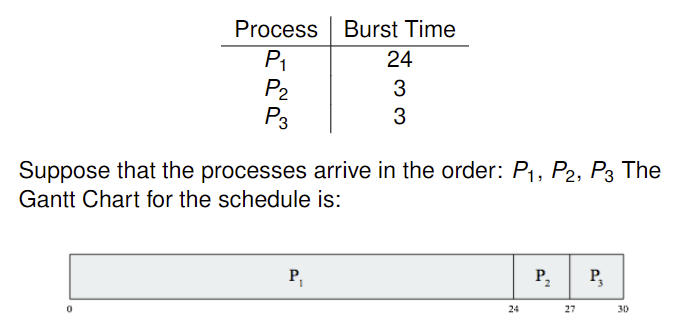
\includegraphics[width=\linewidth]{gantt-chart.png}

    \section{Memory Management}
    \subsection{Paging}
    % this needs to be generalized/changed to not directly be a question
    Given a computer system with a 32-bit logical address and 8-KB page
    size and supports 1 GB of physical memory, how many entries are in
    (a) a conventional, single level page table and in (b) an inverted
    page table? \\
    (a) The logical address space consists of the bits for the page number
    and the page offset. Each page is 8KB which is $2^{13}$ bytes, so 13 bits
    are needed for the page offset. As 32-13 = 19, 19 bits are used for
    the page number and thus the page table can have $2^{19}$ entries. \\
    (b) Inverted page tables keep only one entry for each real page
    (frame) in memory. 13 bits are still kept for the page offset, but
    we subtract from  the number of bits used for the physical memory,
    which is 30 (since \(\qty{1}{\giga\byte} = \qty[parse-numbers=false]{2^{30}}{\byte}\)).
    30-13 = 17, thus the
    number of entries would be $2^{17}$.
    \section{Virtual Memory}
    \subsection{Demand Paging}
    $\text{\textbf{effective access time}} = (1-p) \cdot ma + p \cdot \text
        {page fault time}$ where $p$ is the probability of a page fault and $ma$
    is the memory access time.
    \section{File System}
    Logic for ``answering maximum size of file'' type questions: multiply the
    number of direct disk blocks by size of the disk blocks, for indirect
    disk blocks, divide the size of the disk blocks by the size of a pointer to
    a disk block, then raise this number by a power which is the same as the
    level of the indirect block (i.e. for single indirect raise by a power of
    1, for a double indirect raise by a power of 2, and so on).
    Multiply this value
    by the size of a disk block and by the amount of that specific indirect
    disk block, i.e. if you are doing the calculation for 5 single indirect
    disk blocks, then multiply by 5 at the end. Add the multiplications
    for all the types of disk blocks together for the final answer.

    \textbf{Volume:} disk block that contains file system.

    Logic for ``answering maximum size of file'' type questions: multiply the
    number of direct disk blocks by size of the disk blocks, for indirect
    disk blocks, divide the size of the disk blocks by the size of a pointer to
    a disk block, then raise this number by a power which is the same as the
    level of the indirect block (i.e. for single indirect raise by a power of
    1, for a double indirect raise by a power of 2, and so on).
    Multiply this value
    by the size of a disk block and by the amount of that specific indirect
    disk block, i.e. if you are doing the calculation for 5 single indirect
    disk blocks, then multiply by 5 at the end. Add the multiplications
    for all the types of disk blocks together for the final answer.
    \section{Mass Storage Systems}
    \subsection{SCAN Scheduling}
    The disk arm starts at one end of the disk and moves
    toward the other end, servicing requests as it reaches each cylinder,
    until it gets to the other end of the disk. At the other end, the
    direction of head movement is reversed, and servicing continues
    \subsection{C-SCAN Scheduling}
    C-SCAN moves the head from one end of
    the disk to the other, servicing requests along the way. When the
    head reaches the other end, however, it immediately returns
    to the beginning of the disk without servicing any requests on the
    return trip. Is a variant of SCAN scheduling.
    \section{Conversions}
    \qty{1}{\second} = \qty{1000}{\milli\second},
    \qty{1}{\milli\second} = \qty{1000}{\micro\second} (microsecond),
    \qty{1}{\micro\second} = \qty{1000}{\nano\second}

    \qty{1}{\kilo\byte} = \qty[parse-numbers=false]{2^{10}}{\byte},
    \qty{1}{\mega\byte} = \qty[parse-numbers=false]{2^{20}}{\byte},
    \qty{1}{\giga\byte} = \qty[parse-numbers=false]{2^{30}}{\byte}
    % Previous final and lecture questions that I managed to put in without copying the whole thing word for word. Omitted ez questions that is just plugging formulas. Might need additional formatting.
    % \section{Techniques for Predicted Questions}

\end{multicols*}
\end{document}
